
\section{Detailed Cases:}
\begin{itemize}
  \item Author: Cao Ngoc Anh Tuan
  \item Date: May 30, 2026
  \item System: Breadit Social Web Platform
\end{itemize}

This document contains comprehensive test cases for the Breadit system, covering all major features and workflows based on actual system implementation.

Reference Test Accounts:
\begin{itemize}
  \item User:     user1@example.com / password
  \item Admin:    admin@breadit.dev / 123456
  \item Mod Community
\end{itemize}

\subsection{Authentication \& Account Verification}

This section demonstrates the core authentication flows. Registration and login are the entry points for all platform features. These endpoints are rate-limited (@Throttle: 10 requests per 60 seconds) and use bcrypt for secure password handling.

\subsubsection{Test Case \#: UC01}
\begin{itemize}
  \item Test Case Name: Register Account
  \item System: Breadit
  \item Subsystem: Authentication \& account verification
  \item Short Description:
  \item User registers a new account by providing a unique username, email address, and a strong password. The system validates all inputs, hashes the password with bcrypt (10 salt rounds), and dispatches a 6-digit OTP to the provided email.
  \item Pre-conditions:
  \item No existing account with the provided email or username in the database
  \item SMTP email service is configured in the backend environment
  \item The /sign-up page is accessible
\end{itemize}

\begin{longtable}{|p{0.18\linewidth}|p{0.18\linewidth}|p{0.18\linewidth}|p{0.18\linewidth}|p{0.18\linewidth}|}
\caption{UC01} \label{tab:27} \\
\hline
\textbf{Step} & \textbf{Action} & \textbf{System Response} & \textbf{Pass/Fail} & \textbf{Comments} \\
\hline
\endfirsthead
\multicolumn{5}{l}{\textit{(Continued from previous page)}} \\
\hline
\textbf{Step} & \textbf{Action} & \textbf{System Response} & \textbf{Pass/Fail} & \textbf{Comments} \\
\hline
\endhead
\hline \multicolumn{5}{r}{\textit{Continued on next page}} \\
\endfoot
\hline
\endlastfoot
01 & Submit registration form at /sign-up & Calls register API & Pass &  \\
\hline
02 & System validates inputs & Checks format and password strength & Pass &  \\
\hline
03 & System checks duplicate & Queries DB (returns 409 if duplicate) & Pass &  \\
\hline
04 & System hashes passwords and saves users with emailVerified: null & bcrypt (10 rounds); saves User record & Pass & Bcrypt 10 rounds \\
\hline
05 & System sends OTP \& redirects & Stores token, sends email, redirects & Pass & OTP valid for 15m \\
\hline
\end{longtable}

\begin{itemize}
  \item Post-condition:
  \item A new~User~record exists in the database with~emailVerified = null
  \item A VerificationToken~row is stored
  \item User's inbox contains a verification email with the 6-digit OTP
\end{itemize}

\subsubsection{Test Case \#: UC04}
\begin{itemize}
  \item Test Case Name: Log In with Email and Password
  \item System: Breadit
  \item Subsystem: Authentication \& Account Verification
  \item Short Description:
\begin{itemize}
  \item User logs into the system using a registered email and password. The system validates credentials via bcrypt comparison and issues a JWT breadit\_session httpOnly cookie on success.
\end{itemize}
  \item Pre-conditions:
\begin{itemize}
  \item A user account with the provided email exists in the database
  \item User's email is verified (emailVerified is not null)
  \item The /sign-in page is accessible
\end{itemize}
\end{itemize}

\begin{longtable}{|p{0.18\linewidth}|p{0.18\linewidth}|p{0.18\linewidth}|p{0.18\linewidth}|p{0.18\linewidth}|}
\caption{UC04} \label{tab:28} \\
\hline
\textbf{Step} & \textbf{Action} & \textbf{System Response} & \textbf{Pass/Fail} & \textbf{Comments} \\
\hline
\endfirsthead
\multicolumn{5}{l}{\textit{(Continued from previous page)}} \\
\hline
\textbf{Step} & \textbf{Action} & \textbf{System Response} & \textbf{Pass/Fail} & \textbf{Comments} \\
\hline
\endhead
\hline \multicolumn{5}{r}{\textit{Continued on next page}} \\
\endfoot
\hline
\endlastfoot
01 & Submit credentials at /sign-in & Calls login API & Pass &  \\
\hline
02 & System queries user & Finds user by email & Pass &  \\
\hline
03 & System compares password & Compares bcrypt hash & Pass &  \\
\hline
04 & System generates JWT & Creates token with claims & Pass &  \\
\hline
05 & System sets session cookie & Sets breadit\_session cookie & Pass & httpOnly cookie \\
\hline
06 & System redirects to / & Redirects to homepage / & Pass &  \\
\hline
\end{longtable}

\begin{itemize}
  \item Post-condition:
\begin{itemize}
  \item Users can access all protected routes.
  \item User is redirected to the home feed at /
\end{itemize}
\end{itemize}

\subsection{Feeds \& Discovery}

This section demonstrates how users discover content. The home feed shows posts from followed users; the explore feed surfaces trending content ranked by a time-decay engagement algorithm with author-diversity enforcement. Global search spans posts, users, hashtags, and communities.

\subsubsection{Test Case \#: UC26}
\begin{itemize}
  \item Test Case Name: View Home Feed (For You)
  \item System: Breadit
  \item Subsystem: Feeds \& Discovery
  \item Short Description:
\begin{itemize}
  \item Authenticated user views a personalized home feed containing top-level posts from themselves and followed users, ordered by most recent. Community posts and replies are excluded. Blocked users are filtered out.
\end{itemize}
  \item Pre-conditions:
\begin{itemize}
  \item User is authenticated.
  \item User follows at least one other user who has published posts.
  \item Posts exist in the system.
\end{itemize}
\end{itemize}

\begin{longtable}{|p{0.18\linewidth}|p{0.18\linewidth}|p{0.18\linewidth}|p{0.18\linewidth}|p{0.18\linewidth}|}
\caption{UC26} \label{tab:29} \\
\hline
\textbf{Step} & \textbf{Action} & \textbf{System Response} & \textbf{Pass/Fail} & \textbf{Comments} \\
\hline
\endfirsthead
\multicolumn{5}{l}{\textit{(Continued from previous page)}} \\
\hline
\textbf{Step} & \textbf{Action} & \textbf{System Response} & \textbf{Pass/Fail} & \textbf{Comments} \\
\hline
\endhead
\hline \multicolumn{5}{r}{\textit{Continued on next page}} \\
\endfoot
\hline
\endlastfoot
01 & Click "For you" or navigate to / & Calls feed API with token & Pass &  \\
\hline
02 & System validates request & Optional\allowbreak{}Jwt\allowbreak{}Auth\allowbreak{}Guard checks auth & Pass &  \\
\hline
03 & System filters posts & Queries posts from self/followees & Pass & Exclude replies \\
\hline
04 & System sorts and paginates & Orders createdAt desc (limit 3) & Pass &  \\
\hline
05 & Frontend displays feed & Renders post list with scroll pagination & Pass &  \\
\hline
\end{longtable}

\begin{itemize}
  \item Post-condition:
\begin{itemize}
  \item Users see a personalized feed sorted by most recent.
  \item Interaction state (liked, saved, reposted) is correct per post.
\end{itemize}
\end{itemize}

\subsubsection{Test Case \#: UC27}
\begin{itemize}
  \item Test Case Name: View Explore Feed (Discover)
  \item System: Breadit
  \item Subsystem: Feeds \& Discovery
  \item Short Description:
\begin{itemize}
  \item User views the explore feed, which surfaces globally trending posts ranked by a time-decay engagement score. Author-diversity is enforced.
\end{itemize}
  \item Pre-conditions:
\begin{itemize}
  \item Posts exist in the system created within the last 7 days.
  \item User may be authenticated or a guest.
\end{itemize}
\end{itemize}

\begin{longtable}{|p{0.18\linewidth}|p{0.18\linewidth}|p{0.18\linewidth}|p{0.18\linewidth}|p{0.18\linewidth}|}
\caption{UC27} \label{tab:30} \\
\hline
\textbf{Step} & \textbf{Action} & \textbf{System Response} & \textbf{Pass/Fail} & \textbf{Comments} \\
\hline
\endfirsthead
\multicolumn{5}{l}{\textit{(Continued from previous page)}} \\
\hline
\textbf{Step} & \textbf{Action} & \textbf{System Response} & \textbf{Pass/Fail} & \textbf{Comments} \\
\hline
\endhead
\hline \multicolumn{5}{r}{\textit{Continued on next page}} \\
\endfoot
\hline
\endlastfoot
01 & Click "Explore" tab & Calls explore feed API & Pass &  \\
\hline
02 & System filters posts & Gets top-level posts from last 7 days & Pass & Last 7 days posts \\
\hline
03 & System computes scores & Calculates time-decay score & Pass &  \\
\hline
04 & System applies diversity cap & Restricts to max 3 posts per author & Pass & Max 3 posts/author \\
\hline
05 & System paginates feed & Returns ranked posts with cursor & Pass &  \\
\hline
06 & Frontend displays posts & Renders explore feed; loads on scroll & Pass &  \\
\hline
\end{longtable}

\begin{itemize}
  \item Post-condition:
\begin{itemize}
  \item User sees a trending feed ranked by engagement quality.
\end{itemize}
\end{itemize}

\subsubsection{Test Case \#: UC30}
\begin{itemize}
  \item Test Case Name: Global Search
  \item System: Breadit
  \item Subsystem: Feeds \& Discovery
  \item Short Description:
\begin{itemize}
  \item User submits a search query and receives multi-type results: matching posts, users, hashtags, and communities (up to 5 each). Queries run in parallel; results are block-filtered for authenticated users.
\end{itemize}
  \item Pre-conditions:
\begin{itemize}
  \item Search query string q is non-empty (at least 1 character)
  \item Users may be authenticated or a guest.
\end{itemize}
  \item 
\end{itemize}

\begin{longtable}{|p{0.18\linewidth}|p{0.18\linewidth}|p{0.18\linewidth}|p{0.18\linewidth}|p{0.18\linewidth}|}
\caption{UC30} \label{tab:31} \\
\hline
\textbf{Step} & \textbf{Action} & \textbf{System Response} & \textbf{Pass/Fail} & \textbf{Comments} \\
\hline
\endfirsthead
\multicolumn{5}{l}{\textit{(Continued from previous page)}} \\
\hline
\textbf{Step} & \textbf{Action} & \textbf{System Response} & \textbf{Pass/Fail} & \textbf{Comments} \\
\hline
\endhead
\hline \multicolumn{5}{r}{\textit{Continued on next page}} \\
\endfoot
\hline
\endlastfoot
01 & Enter query in search bar & Calls search API & Pass &  \\
\hline
02 & System checks credentials & Optional\allowbreak{}Jwt\allowbreak{}Auth\allowbreak{}Guard runs (guests allowed) & Pass &  \\
\hline
03 & System runs searches & Runs parallel queries on posts, users, tags, communities & Pass & Parallel searches \\
\hline
04 & System groups results & Returns up to 5 items per category & Pass &  \\
\hline
05 & System paginates feed & Returns ranked posts with cursor & Pass &  \\
\hline
06 & Frontend renders results & Displays lists; navigates on click & Pass &  \\
\hline
\end{longtable}

\begin{itemize}
  \item Post-condition:
\begin{itemize}
  \item Multi-type search results displayed in sections.
  \item Clicking a result navigates to the post permalink, user profile, hashtag feed, or community page.
\end{itemize}
\end{itemize}

\subsection{Post Management}

This section covers post creation, editing, and deletion. All post mutations go through a unified multipart endpoint that handles both text content and media files. Soft delete is used to preserve referential integrity.

\subsubsection{Test Case \#: UC08}
\begin{itemize}
  \item Test Case Name: Create Text Post
  \item System: Breadit
  \item Subsystem: Post Management
  \item Short Description:
\begin{itemize}
  \item Authenticated and email-verified user creates a text post from the Share component. The system parses hashtags and @mentions, persists the post, and notifies mentioned users.
\end{itemize}
  \item Pre-conditions:
\begin{itemize}
  \item User is authenticated and email verified.
\end{itemize}
\end{itemize}

\begin{longtable}{|p{0.18\linewidth}|p{0.18\linewidth}|p{0.18\linewidth}|p{0.18\linewidth}|p{0.18\linewidth}|}
\caption{UC08} \label{tab:32} \\
\hline
\textbf{Step} & \textbf{Action} & \textbf{System Response} & \textbf{Pass/Fail} & \textbf{Comments} \\
\hline
\endfirsthead
\multicolumn{5}{l}{\textit{(Continued from previous page)}} \\
\hline
\textbf{Step} & \textbf{Action} & \textbf{System Response} & \textbf{Pass/Fail} & \textbf{Comments} \\
\hline
\endhead
\hline \multicolumn{5}{r}{\textit{Continued on next page}} \\
\endfoot
\hline
\endlastfoot
01 & Write text and click "Post" & Submits multipart request & Pass &  \\
\hline
02 & System checks text length & Validates description & Pass & Max 255 characters \\
\hline
03 & System verifies auth status & Guards check session and verification & Pass &  \\
\hline
04 & System creates Post & Saves Post record to database & Pass &  \\
\hline
05 & System parses hashtags & Creates Hashtag and PostTag rows & Pass & Index hashtags \\
\hline
06 & System parses mention & Sends Socket.IO notifications to mention users & Pass &  \\
\hline
07 & Frontend updates feed & Prepends new post to feed & Pass &  \\
\hline
\end{longtable}

\begin{itemize}
  \item Post-condition:
\begin{itemize}
  \item Post record exists in the database.
  \item \#breadit hashtag is searchable via /hashtag/breadit feed
  \item @alice (if exists) receives a real-time MENTION notification
\end{itemize}
\end{itemize}

\subsubsection{Test Case \#: UC09}
\begin{itemize}
  \item Test Case Name: Create Post with Media (Image/Video)
  \item System: Breadit
  \item Subsystem: Post Management
  \item Short Description:
\begin{itemize}
  \item User attaches image or video files to a post. The system processes each file through Cloudinary (or local sharp fallback) and creates PostMedia rows linked to the post.
\end{itemize}
  \item 
  \item Pre-conditions:
\begin{itemize}
  \item User is authenticated and email-verified
  \item File is a valid image or video format (File size $\leq$ 500 MB per file)
\end{itemize}
\end{itemize}

\begin{longtable}{|p{0.18\linewidth}|p{0.18\linewidth}|p{0.18\linewidth}|p{0.18\linewidth}|p{0.18\linewidth}|}
\caption{UC09} \label{tab:33} \\
\hline
\textbf{Step} & \textbf{Action} & \textbf{System Response} & \textbf{Pass/Fail} & \textbf{Comments} \\
\hline
\endfirsthead
\multicolumn{5}{l}{\textit{(Continued from previous page)}} \\
\hline
\textbf{Step} & \textbf{Action} & \textbf{System Response} & \textbf{Pass/Fail} & \textbf{Comments} \\
\hline
\endhead
\hline \multicolumn{5}{r}{\textit{Continued on next page}} \\
\endfoot
\hline
\endlastfoot
01 & Attach files and click "Post" & Submits multipart request & Pass & Max 10 files, $\leq$ 500MB \\
\hline
02 & System validates files & Checks file size and mime types & Pass &  \\
\hline
03 & System uploads files & Saves to Cloudinary or falls back to Sharp & Pass &  \\
\hline
04 & System creates Post & Saves Post record to database & Pass & Association rules \\
\hline
05 & System creates PostMedia & Links media URLs to Post row & Pass &  \\
\hline
06 & Frontend renders media & Displays post with media grid & Pass &  \\
\hline
\end{longtable}

\begin{itemize}
  \item Post-condition:
\begin{itemize}
  \item Post and PostMedia records exist in the database.
  \item Posts with media are visible in the feed.
\end{itemize}
  \item 
\end{itemize}

\subsection{Post Interaction}

This section covers user engagement actions: liking, commenting (replying), reposting, and bookmarking. All interaction endpoints require authentication; most also require email verification and a non-banned account status.

\subsubsection{Test Case \#: UC15}
\begin{itemize}
  \item Test Case Name: Like / Unlike Post
  \item System: Breadit
  \item Subsystem: Post Interaction
  \item Short Description:
\begin{itemize}
  \item Authenticated user toggles the like state on a post. A LIKE notification is emitted via Socket.IO to the post owner on first like. Clicking again removes the like.
\end{itemize}
  \item Pre-conditions:
\begin{itemize}
  \item User is authenticated, email-verified, and not banned.
  \item Post exists and is not deleted.
\end{itemize}
\end{itemize}

\begin{longtable}{|p{0.18\linewidth}|p{0.18\linewidth}|p{0.18\linewidth}|p{0.18\linewidth}|p{0.18\linewidth}|}
\caption{UC15} \label{tab:34} \\
\hline
\textbf{Step} & \textbf{Action} & \textbf{System Response} & \textbf{Pass/Fail} & \textbf{Comments} \\
\hline
\endfirsthead
\multicolumn{5}{l}{\textit{(Continued from previous page)}} \\
\hline
\textbf{Step} & \textbf{Action} & \textbf{System Response} & \textbf{Pass/Fail} & \textbf{Comments} \\
\hline
\endhead
\hline \multicolumn{5}{r}{\textit{Continued on next page}} \\
\endfoot
\hline
\endlastfoot
01 & Click heart icon on post & Calls like API & Pass &  \\
\hline
02 & System verifies auth & Checks auth, verification, and ban status & Pass &  \\
\hline
03 & System checks current like & Queries Like table for user/post & Pass &  \\
\hline
04 & System toggles Like row & Deletes (unlike) or inserts (like) & Pass &  \\
\hline
05 & System sends notification & Emits Socket.IO notification to owner & Pass & Notify post owner \\
\hline
06 & Frontend updates button & Toggles heart fill and counter & Pass &  \\
\hline
\end{longtable}

\begin{itemize}
  \item Post-condition:
\begin{itemize}
  \item Like rows exist in the database
  \item Post owner receives a real-time LIKE notification (if actor $\neq$ owner)
  \item Heart icon is filled; like count incremented by 1.
\end{itemize}
\end{itemize}

\subsubsection{Test Case \#: UC10}
\begin{itemize}
  \item Test Case Name: Create Reply / Comment
  \item System: Breadit
  \item Subsystem: Post Interaction
  \item Short Description:
\begin{itemize}
  \item User replies to an existing post, creating a threaded comment. The parent post owner receives a REPLY notification. Replies support text and media attachments.
\end{itemize}
  \item Pre-conditions:
\begin{itemize}
  \item Parent posts exist and is not deleted.
\end{itemize}
\end{itemize}

\begin{longtable}{|p{0.18\linewidth}|p{0.18\linewidth}|p{0.18\linewidth}|p{0.18\linewidth}|p{0.18\linewidth}|}
\caption{UC10} \label{tab:35} \\
\hline
\textbf{Step} & \textbf{Action} & \textbf{System Response} & \textbf{Pass/Fail} & \textbf{Comments} \\
\hline
\endfirsthead
\multicolumn{5}{l}{\textit{(Continued from previous page)}} \\
\hline
\textbf{Step} & \textbf{Action} & \textbf{System Response} & \textbf{Pass/Fail} & \textbf{Comments} \\
\hline
\endhead
\hline \multicolumn{5}{r}{\textit{Continued on next page}} \\
\endfoot
\hline
\endlastfoot
01 & Type reply and click "Reply" & Calls posts API with parent ID & Pass &  \\
\hline
02 & System saves reply & Creates reply post; processes media & Pass & Link parent post ID \\
\hline
03 & System sends notification & Emits Socket.IO notification to parent owner & Pass &  \\
\hline
04 & System parses mention & Dispatches notifications to mentioned users & Pass &  \\
\hline
05 & Frontend appends reply & Displays reply in comment thread & Pass &  \\
\hline
\end{longtable}

\begin{itemize}
  \item Post-condition:
\begin{itemize}
  \item Post record with parentPostId set exists in the database.
  \item Parent post owner receives a real-time REPLY notification.
  \item Reply is visible in the comment thread below the parent post.
\end{itemize}
\end{itemize}

\subsection{User Relationship Management}

This section covers the social graph features: following users to customize the home timeline and blocking users to restrict access. Both operations include real-time feedback and cache invalidation.

\subsubsection{Test Case \#: UC18}
\begin{itemize}
  \item Test Case Name: Follow / Unfollow User
  \item System: Breadit
  \item Subsystem: User Relationship Management
  \item Short Description:
\begin{itemize}
  \item User follows another user to add their posts to the home feed. The target user receives a real-time FOLLOW notification. Clicking the button again unfollows and removes the relationship.
\end{itemize}
  \item Pre-conditions:
\begin{itemize}
  \item Follower is authenticated and not banned.
  \item Follower is viewing the target user's profile page.
\end{itemize}
\end{itemize}

\begin{longtable}{|p{0.18\linewidth}|p{0.18\linewidth}|p{0.18\linewidth}|p{0.18\linewidth}|p{0.18\linewidth}|}
\caption{UC18} \label{tab:36} \\
\hline
\textbf{Step} & \textbf{Action} & \textbf{System Response} & \textbf{Pass/Fail} & \textbf{Comments} \\
\hline
\endfirsthead
\multicolumn{5}{l}{\textit{(Continued from previous page)}} \\
\hline
\textbf{Step} & \textbf{Action} & \textbf{System Response} & \textbf{Pass/Fail} & \textbf{Comments} \\
\hline
\endhead
\hline \multicolumn{5}{r}{\textit{Continued on next page}} \\
\endfoot
\hline
\endlastfoot
01 & Click "Follow" on profile & Calls follow API & Pass &  \\
\hline
02 & System verifies auth & Guards check session and ban status & Pass &  \\
\hline
03 & System checks follow & Queries Follow table & Pass &  \\
\hline
04 & System toggles Follow & Inserts follow row or delete it & Pass &  \\
\hline
05 & System sends notification & Emits Socket.IO notification to target & Pass & Real-time follow notification \\
\hline
06 & Home feed cache updates & Home feed cache updates & Pass &  \\
\hline
\end{longtable}

\begin{itemize}
  \item Post-condition:
\begin{itemize}
  \item Follow row exists in the database.
  \item Target user's posts now appear in the follower's home feed.
  \item Target user received a FOLLOW notification.
\end{itemize}
\end{itemize}

\subsubsection{Test Case \#: UC21}
\begin{itemize}
  \item Test Case Name: Block / Unblock User
  \item System: Breadit
  \item Subsystem: User Relationship Management
  \item Short Description:
\begin{itemize}
  \item User blocks another user, removing all mutual follow relationships and filtering the blocked user from all feeds, search results, and notifications. The block is bidirectional.
\end{itemize}
  \item Pre-conditions:
\begin{itemize}
  \item Acting users are authenticated and not banned.
\end{itemize}
\end{itemize}

\begin{longtable}{|p{0.18\linewidth}|p{0.18\linewidth}|p{0.18\linewidth}|p{0.18\linewidth}|p{0.18\linewidth}|}
\caption{UC21} \label{tab:37} \\
\hline
\textbf{Step} & \textbf{Action} & \textbf{System Response} & \textbf{Pass/Fail} & \textbf{Comments} \\
\hline
\endfirsthead
\multicolumn{5}{l}{\textit{(Continued from previous page)}} \\
\hline
\textbf{Step} & \textbf{Action} & \textbf{System Response} & \textbf{Pass/Fail} & \textbf{Comments} \\
\hline
\endhead
\hline \multicolumn{5}{r}{\textit{Continued on next page}} \\
\endfoot
\hline
\endlastfoot
01 & Select "Block" on profile & Calls block API & Pass &  \\
\hline
02 & System verifies auth & Guards check session and ban status & Pass &  \\
\hline
03 & System checks block & Queries Block table & Pass &  \\
\hline
04 & System toggles Block & Inserts block row or delete it & Pass &  \\
\hline
05 & System removes follows & Deletes mutual follows in both directions & Pass & Delete mutual follows \\
\hline
06 & System filters content & Bidirectionally filters posts and search & Pass & Bidirectional \\
\hline
\end{longtable}

\begin{itemize}
  \item Post-condition:
\begin{itemize}
  \item Block row exists in the database.
  \item All mutual Follow relationships are deleted.
  \item Blocked user is excluded from feeds, search, and notifications.
\end{itemize}
\end{itemize}

\subsection{Profile Management}

This section covers profile viewing and editing. Profiles are rendered via Server-Side Rendering and include block-status checks. Profile updates use a sparse PATCH operation so only provided fields are modified.

\subsubsection{Test Case \#: UC22}
\begin{itemize}
  \item Test Case Name: View User Profile
  \item System: Breadit
  \item Subsystem: Profile Management
\end{itemize}
\begin{itemize}
  \item Short Description:
\begin{itemize}
  \item User navigates to another user's profile. The system checks block status in both directions, returns the full profile with follower/following counts, interaction options.
\end{itemize}
  \item Pre-conditions:
\begin{itemize}
  \item Target users exist and are not banned.
\end{itemize}
\end{itemize}

\begin{longtable}{|p{0.18\linewidth}|p{0.18\linewidth}|p{0.18\linewidth}|p{0.18\linewidth}|p{0.18\linewidth}|}
\caption{UC22} \label{tab:38} \\
\hline
\textbf{Step} & \textbf{Action} & \textbf{System Response} & \textbf{Pass/Fail} & \textbf{Comments} \\
\hline
\endfirsthead
\multicolumn{5}{l}{\textit{(Continued from previous page)}} \\
\hline
\textbf{Step} & \textbf{Action} & \textbf{System Response} & \textbf{Pass/Fail} & \textbf{Comments} \\
\hline
\endhead
\hline \multicolumn{5}{r}{\textit{Continued on next page}} \\
\endfoot
\hline
\endlastfoot
01 & Navigate to profile /: username & Initiates profile load & Pass &  \\
\hline
02 & System fetches user profile & Calls user detail API & Pass &  \\
\hline
03 & System checks block & Queries database for mutual block & Pass &  \\
\hline
04 & System restricts view & Returns basic details only if blocked & Pass & Restrict post view \\
\hline
05 & System returns full profile & Returns profile fields, counts, and posts & Pass &  \\
\hline
06 & Frontend displays profile & Renders header, actions, and tabs & Pass &  \\
\hline
\end{longtable}

\begin{itemize}
  \item Post-condition:
\begin{itemize}
  \item Viewers can follow, block, message, or browse the target's posts via tabs.
\end{itemize}
  \item 
\end{itemize}

\subsection{Direct Messaging}

This section covers 1:1 real-time messaging. Conversations persisted in the database and delivered in real-time via Socket.IO. Unread message counts are tracked per conversation and displayed as a badge in the sidebar.

\subsubsection{Test Case \#: UC40}
\begin{itemize}
  \item Test Case Name: Start or Find a Conversation
  \item System: Breadit
  \item Subsystem: Direct Messaging
  \item Short Description:
\begin{itemize}
  \item User initiates a direct message thread with another user. If a conversation already exists between the two, the system returns it; otherwise, a new one is created.
\end{itemize}
  \item Pre-conditions:
\begin{itemize}
  \item Initiating user is authenticated and email verified.
\end{itemize}
  \item 
\end{itemize}

\begin{longtable}{|p{0.18\linewidth}|p{0.18\linewidth}|p{0.18\linewidth}|p{0.18\linewidth}|p{0.18\linewidth}|}
\caption{UC40} \label{tab:39} \\
\hline
\textbf{Step} & \textbf{Action} & \textbf{System Response} & \textbf{Pass/Fail} & \textbf{Comments} \\
\hline
\endfirsthead
\multicolumn{5}{l}{\textit{(Continued from previous page)}} \\
\hline
\textbf{Step} & \textbf{Action} & \textbf{System Response} & \textbf{Pass/Fail} & \textbf{Comments} \\
\hline
\endhead
\hline \multicolumn{5}{r}{\textit{Continued on next page}} \\
\endfoot
\hline
\endlastfoot
01 & Click Message on profile & Calls conversation API & Pass &  \\
\hline
02 & System verifies credentials & Guards check session and verification & Pass &  \\
\hline
03 & System checks user ID & Confirms user is not messaging self & Pass &  \\
\hline
04 & System searches conversation & Queries database for existing pair & Pass &  \\
\hline
05 & System returns conversation & Returns metadata if conversation exists & Pass &  \\
\hline
06 & System creates conversation & Atomically inserts conversation \& member rows & Pass &  \\
\hline
07 & Frontend redirects & Navigates to /messages/:id & Pass & Redirect to thread \\
\hline
\end{longtable}

\begin{itemize}
  \item Post-condition:
\begin{itemize}
  \item Conversation and two ConversationMember rows exist in the database.
  \item User is navigated to the message thread at /messages/: conversationId
\end{itemize}
\end{itemize}

\subsubsection{Test Case \#: UC43}
\begin{itemize}
  \item Test Case Name: Send Text Message
  \item System: Breadit
  \item Subsystem: Direct Messaging
  \item Short Description:
\begin{itemize}
  \item User sends a text message in a conversation. The message persisted and delivered to the recipient in real-time via Socket.IO. The conversation is bumped to the top of both users' lists.
\end{itemize}
  \item Pre-conditions:
\begin{itemize}
  \item User is authenticated and email verified.
  \item User is a ConversationMember of the target conversation.
\end{itemize}
\end{itemize}

\begin{longtable}{|p{0.18\linewidth}|p{0.18\linewidth}|p{0.18\linewidth}|p{0.18\linewidth}|p{0.18\linewidth}|}
\caption{UC43} \label{tab:40} \\
\hline
\textbf{Step} & \textbf{Action} & \textbf{System Response} & \textbf{Pass/Fail} & \textbf{Comments} \\
\hline
\endfirsthead
\multicolumn{5}{l}{\textit{(Continued from previous page)}} \\
\hline
\textbf{Step} & \textbf{Action} & \textbf{System Response} & \textbf{Pass/Fail} & \textbf{Comments} \\
\hline
\endhead
\hline \multicolumn{5}{r}{\textit{Continued on next page}} \\
\endfoot
\hline
\endlastfoot
01 & Type message and click Send & Inputs text (checks $\leq$ 1000 limit) & Pass &  \\
\hline
02 & Frontend appends message & Renders message instantly in chat UI & Pass &  \\
\hline
03 & System checks credentials & Guards check auth, verification, \& member role & Pass &  \\
\hline
04 & System saves message & Inserts Message row in DB & Pass &  \\
\hline
05 & System sends message & Emits newMessage Socket.IO event & Pass & Socket.IO broadcast \\
\hline
06 & System updates activity time & Refreshes Conversation.updatedAt timestamp & Pass &  \\
\hline
07 & System returns message & Returns saved row; swaps UI card & Pass &  \\
\hline
\end{longtable}

\begin{itemize}
  \item Post-condition:
\begin{itemize}
  \item Message row persisted in the database
  \item Recipient receives the message in real-time via Socket.IO.
  \item Conversation updatedAt is refreshed; conversation appears at the top of both users' lists.
\end{itemize}
\end{itemize}

\subsection{Real-time Notifications}

This section covers the notification system. Notifications for likes, replies, reposts, follows, and mentions persisted in the database and pushed in real-time via Socket.IO. Redis is used to scale broadcasting across multiple server instances.

\subsubsection{Test Case \#: UC37}
\begin{itemize}
  \item Test Case Name: View Notification List
  \item System: Breadit
  \item Subsystem: Real-time Notifications
  \item Short Description:
\begin{itemize}
  \item Authenticated user views their paginated notification history. Notifications include LIKE, REPLY, REPOST, FOLLOW, MENTION, and COMMUNITY types with read/unread visual indicators.
\end{itemize}
  \item Pre-conditions:
\begin{itemize}
  \item At least one notification exists for the user.
\end{itemize}
\end{itemize}

\begin{longtable}{|p{0.18\linewidth}|p{0.18\linewidth}|p{0.18\linewidth}|p{0.18\linewidth}|p{0.18\linewidth}|}
\caption{UC37} \label{tab:41} \\
\hline
\textbf{Step} & \textbf{Action} & \textbf{System Response} & \textbf{Pass/Fail} & \textbf{Comments} \\
\hline
\endfirsthead
\multicolumn{5}{l}{\textit{(Continued from previous page)}} \\
\hline
\textbf{Step} & \textbf{Action} & \textbf{System Response} & \textbf{Pass/Fail} & \textbf{Comments} \\
\hline
\endhead
\hline \multicolumn{5}{r}{\textit{Continued on next page}} \\
\endfoot
\hline
\endlastfoot
01 & Click notifications bell icon & Calls notifications API & Pass &  \\
\hline
02 & System validates user session & JwtAuthGuard checks credentials & Pass &  \\
\hline
03 & System queries notifications & Fetches user notifications with details & Pass &  \\
\hline
04 & System sorts and paginates & Orders by createdAt desc & Pass & Sort desc, limit 10 \\
\hline
05 & System returns lists & Returns items; frontend renders list & Pass &  \\
\hline
06 & Click notification & Calls read API; marks record; navigates & Pass &  \\
\hline
\end{longtable}

\begin{itemize}
  \item Post-condition:
\begin{itemize}
  \item Full notification history is visible to the user.
  \item Clicked notifications are marked as read (readAt set)
\end{itemize}
\end{itemize}

\subsection{Community Management}

This section covers the community lifecycle: creation, membership, and content moderation. Communities use a role hierarchy (OWNER $\rightarrow$ MOD $\rightarrow$ MEMBER). Member posts enter a moderation queue and require approval before becoming visible in the community feed.

\subsubsection{Test Case \#: UC51}
\begin{itemize}
  \item Test Case Name: Approve / Reject Community Post
  \item System: Breadit
  \item Subsystem: Community Management
  \item Short Description:
\begin{itemize}
  \item Community OWNER or MOD reviews a pending post submitted by a MEMBER. Approving publishes the post to the community feed and notifies all members. Rejecting soft deletes the post.
\end{itemize}
  \item Pre-conditions:
\begin{itemize}
  \item At least one post with isApproved = false exists in the community
  \item Acting users are authenticated and have OWNER or MOD role in the community.
\end{itemize}
  \item 
\end{itemize}

\begin{longtable}{|p{0.18\linewidth}|p{0.18\linewidth}|p{0.18\linewidth}|p{0.18\linewidth}|p{0.18\linewidth}|}
\caption{UC51} \label{tab:42} \\
\hline
\textbf{Step} & \textbf{Action} & \textbf{System Response} & \textbf{Pass/Fail} & \textbf{Comments} \\
\hline
\endfirsthead
\multicolumn{5}{l}{\textit{(Continued from previous page)}} \\
\hline
\textbf{Step} & \textbf{Action} & \textbf{System Response} & \textbf{Pass/Fail} & \textbf{Comments} \\
\hline
\endhead
\hline \multicolumn{5}{r}{\textit{Continued on next page}} \\
\endfoot
\hline
\endlastfoot
01 & Moderator clicks Approve/Reject & Calls moderate API & Pass &  \\
\hline
02 & System verifies role & Checks if role is OWNER or MOD & Pass & Verify OWNER/MOD role \\
\hline
03 & System updates post & Sets isApproved = true or soft-deletes post & Pass &  \\
\hline
04 & System sends notification & Emits COMMUNITY\_NEW\_POST event & Pass &  \\
\hline
05 & System returns state & Removes post from queue; updates feed & Pass &  \\
\hline
\end{longtable}


\subsection{Administrative Moderation}

This section covers the admin console features. Administrators have site-wide authority to manage users (ban/unban) and handle content reports. All admin routes are protected by both JwtAuthGuard and RolesGuard requiring role = ADMIN.

\subsubsection{Test Case \#: UC62}
\begin{itemize}
  \item Test Case Name: Ban / Unban User (Admin)
  \item System: Breadit
  \item Subsystem: Administrative Moderation
  \item Short Description:
\begin{itemize}
  \item Administrator bans a user from the platform. The BannedUserGuard on all write endpoints will subsequently block any write action attempted by the banned user.
\end{itemize}
  \item Pre-conditions:
\begin{itemize}
  \item Acting user has role = ADMIN
\end{itemize}
\end{itemize}

\begin{longtable}{|p{0.18\linewidth}|p{0.18\linewidth}|p{0.18\linewidth}|p{0.18\linewidth}|p{0.18\linewidth}|}
\caption{UC62} \label{tab:43} \\
\hline
\textbf{Step} & \textbf{Action} & \textbf{System Response} & \textbf{Pass/Fail} & \textbf{Comments} \\
\hline
\endfirsthead
\multicolumn{5}{l}{\textit{(Continued from previous page)}} \\
\hline
\textbf{Step} & \textbf{Action} & \textbf{System Response} & \textbf{Pass/Fail} & \textbf{Comments} \\
\hline
\endhead
\hline \multicolumn{5}{r}{\textit{Continued on next page}} \\
\endfoot
\hline
\endlastfoot
01 & Admin clicks Ban/Unban & Calls admin ban/unban API & Pass &  \\
\hline
02 & System verifies admin & Guards verify ADMIN role & Pass & Verify ADMIN role \\
\hline
03 & System updates database & Toggles User.banned status & Pass &  \\
\hline
04 & System returns success & Returns ok response; updates table & Pass &  \\
\hline
05 & System restricts user & BannedUserGuard blocks write requests & Pass & Revoke write access \\
\hline
06 & Frontend alerts user & Displays suspension banner on reload & Pass &  \\
\hline
\end{longtable}

\begin{itemize}
  \item Post-condition:
\begin{itemize}
  \item User.banned = true in the database
  \item Banned user cannot perform any write actions (posts, likes, follows, messages{\ldots}
  \item Admin can unban at any time via POST /api/admin/users/:id/unban
\end{itemize}
\end{itemize}

\subsubsection{Test Case \#: UC65}
\begin{itemize}
  \item Test Case Name: Delete Reported Post (Admin)
  \item System: Breadit
  \item Subsystem: Administrative Moderation
  \item Short Description:
\begin{itemize}
  \item Administrator reviews the reports queue and permanently softly deletes a reported post, simultaneously closing the report. Admins receive real-time REPORT notifications via Socket.IO when a new report is submitted.
\end{itemize}
  \item Pre-conditions:
\begin{itemize}
  \item At least one OPEN report exists in the queue (Report.status = "OPEN")
  \item The reported post exists and has not been deleted.
\end{itemize}
\end{itemize}

\begin{longtable}{|p{0.18\linewidth}|p{0.18\linewidth}|p{0.18\linewidth}|p{0.18\linewidth}|p{0.18\linewidth}|}
\caption{UC65} \label{tab:44} \\
\hline
\textbf{Step} & \textbf{Action} & \textbf{System Response} & \textbf{Pass/Fail} & \textbf{Comments} \\
\hline
\endfirsthead
\multicolumn{5}{l}{\textit{(Continued from previous page)}} \\
\hline
\textbf{Step} & \textbf{Action} & \textbf{System Response} & \textbf{Pass/Fail} & \textbf{Comments} \\
\hline
\endhead
\hline \multicolumn{5}{r}{\textit{Continued on next page}} \\
\endfoot
\hline
\endlastfoot
01 & Admin clicks Delete post on report & Calls delete reported post API & Pass &  \\
\hline
02 & System verifies admin role & Guards verify ADMIN role & Pass & Verify ADMIN role \\
\hline
03 & System soft-deletes post & Sets deletedAt = now() in database & Pass & Soft-delete post \\
\hline
04 & System closes report & Sets Report.status = 'CLOSED' in & Pass &  \\
\hline
05 & Frontend updates queue & Removes report card from list & Pass &  \\
\hline
\end{longtable}

\begin{itemize}
  \item Post-condition:
\begin{itemize}
  \item Reported post is soft-deleted (deletedAt set) and hidden from all feeds
  \item Report.status = "CLOSED"; report removed from the admin queue
\end{itemize}
\end{itemize}

\section{Evaluation:}

\subsection{Performance:}

\textbf{Verification method: Quantitative --- Redis INFO telemetry}

After warming the cache with 20 consecutives explore feed requests, Redis telemetry was captured:
\begin{center}
  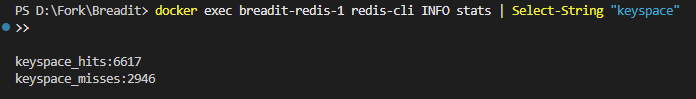
\includegraphics[width=0.92\linewidth,height=0.82\textheight,keepaspectratio]{images/image81.png}
\end{center}

Target: Cache hit rate $\geq$ 70\% under normal load (same query repeated across users)

 Redis cache reduces repeated PostgreSQL reads for trending queries.

\textbf{Verification method:~Quantitative --- k6 load test} (\texttt{docs/planning/k6\_perf\_test.js})

The explore feed endpoint (GET /api/posts?feed=explore) was tested under two scenarios:
\begin{center}
  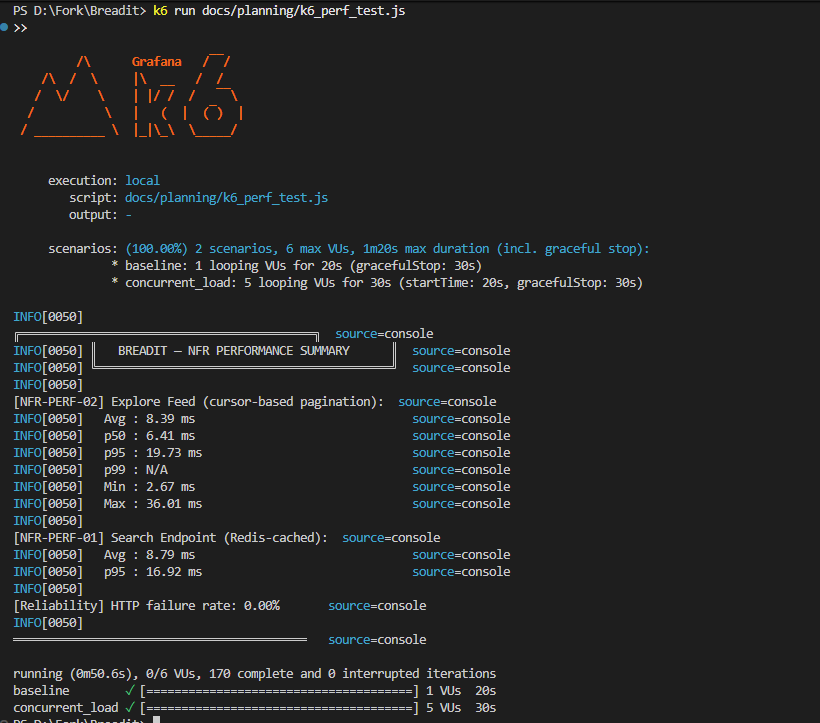
\includegraphics[width=0.92\linewidth,height=0.82\textheight,keepaspectratio]{images/image82.png}
\end{center}
\begin{itemize}
  \item Repeated requests to the same page (cursor) return cached results, observable in the significantly lower p50 vs p95 spread.
  \item Page 2 requests (new cursor) show slightly higher latency due to cache miss on first request, then drop on subsequent identical cursor requests.
\end{itemize}

\subsection{Scalability:}

\textbf{Verification method:~Qualitative + response header inspection}

The~@Throttle~decorator (10 requests per 60 seconds) is applied to authentication endpoints. Exceeding the limit returns HTTP 429 with a~Retry-After~header:
\begin{center}
  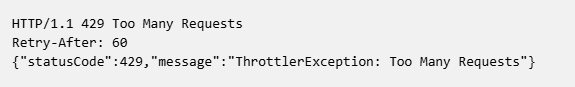
\includegraphics[width=0.92\linewidth,height=0.82\textheight,keepaspectratio]{images/image83.png}
\end{center}

\subsection{Usability:}

\textbf{Verification method:~Quantitative --- Lighthouse audit}

A Lighthouse audit was conducted on the Explore feed page ():
\begin{center}
  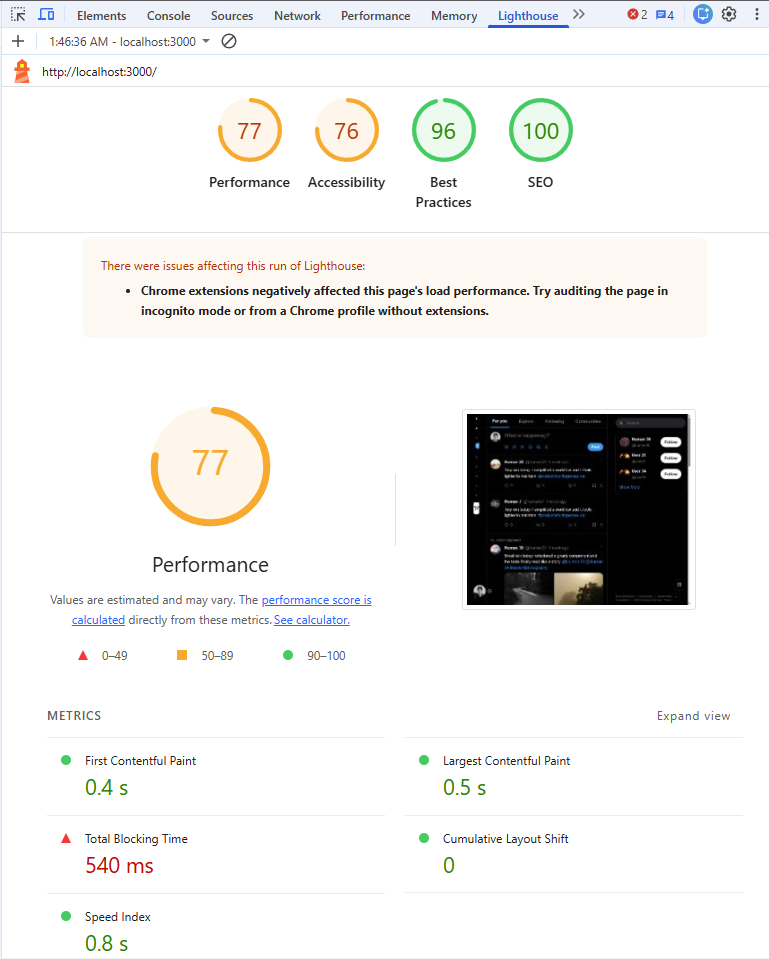
\includegraphics[width=0.92\linewidth,height=0.82\textheight,keepaspectratio]{images/image84.png}
\end{center}

\subsection{Real-Time Performance: WebSocket Notification Latency:}
\begin{center}
  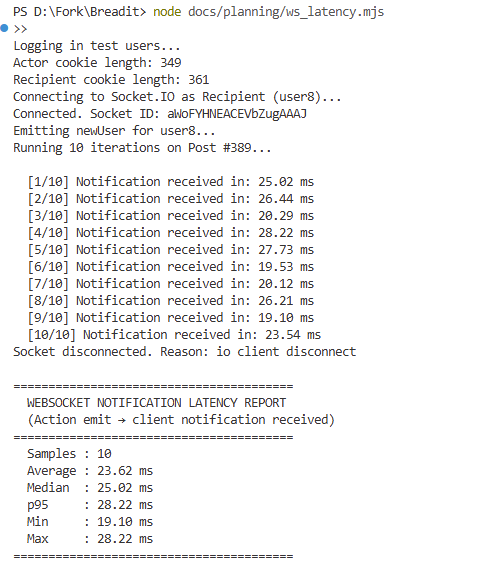
\includegraphics[width=0.92\linewidth,height=0.82\textheight,keepaspectratio]{images/image85.png}
\end{center}

\textbf{Interpretation}: The average end-to-end latency from a user action (like) to the target user's notification event arriving via Socket.IO is 23.62 ms in the local environment. This latency consists of: (1) HTTP request to NestJS $\rightarrow$ (2) database write $\rightarrow$ (3) Socket.IO emit $\rightarrow$ (4) Redis pub/sub broadcast $\rightarrow$ (5) client reception.

\subsection{Content Discovery Algorithm:}

\textbf{Qualitative Comparison: Time-Decay Scoring vs. Like-Count Baseline}

To evaluate whether the time-decay heuristic produces more relevant "trending" results than a naive like-count ranking, the following comparison was conducted using a sample of 10 posts from the local database:
\begin{center}
  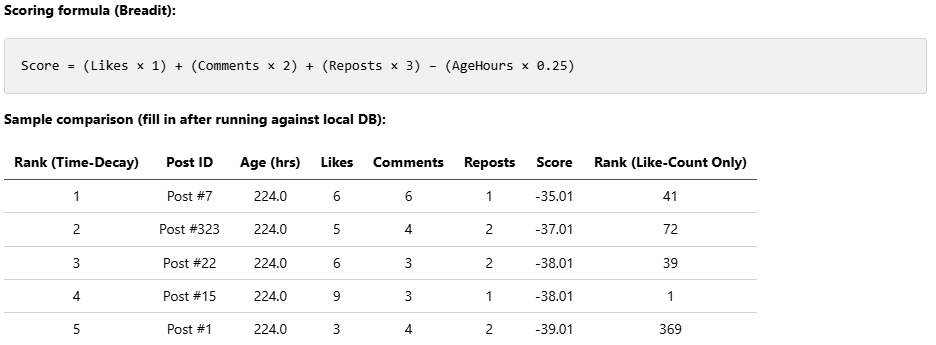
\includegraphics[width=0.92\linewidth,height=0.82\textheight,keepaspectratio]{images/image86.png}
\end{center}
\begin{itemize}
  \item Posts with high like counts but older age are ranked lower under time-decay scoring, ensuring freshness.
  \item Recent posts with moderate engagement appear higher than stale posts with higher total likes.
  \item The author-diversity filter (max 3 posts per author) prevents any single user's content from dominating the feed.
\end{itemize}

\textbf{Result:}~The time-decay heuristic demonstrably surfaces more recent, contextually relevant content compared to a naive like-count baseline, fulfilling the stated content discovery goal.
